%%
%% getstart.tex -- Flight Gear documentation: The FlightGear Manual
%% Title file
%%
%% Written by Michael Basler, started September 1998.
%%
%% Copyright (C) 2002 Michael Basler
%%
%%
%% This program is free software; you can redistribute it and/or
%% modify it under the terms of the GNU General Public License as
%% published by the Free Software Foundation; either version 2 of the
%% License, or (at your option) any later version.
%%
%% This program is distributed in the hope that it will be useful, but
%% WITHOUT ANY WARRANTY; without even the implied warranty of
%% MERCHANTABILITY or FITNESS FOR A PARTICULAR PURPOSE.  See the GNU
%% General Public License for more details.
%%
%% You should have received a copy of the GNU General Public License
%% along with this program; if not, write to the Free Software
%% Foundation, Inc., 675 Mass Ave, Cambridge, MA 02139, USA.
%%
%% $Id: title.tex,v 0.6 2002/09/09 michael
%% (Log is kept at end of this file)

%%%%%%%%%%%%%%%%%%%%%%%%%%%%%%%%%%%%%%%%%%%%%%%%%%%%%%%%%%%%%%%%%%%%%%%%%%%%%%%%%%%%%%%%%%%%%%%
\IfLanguageName{french}{
\title{Le manuel FlightGear}
}{}
\IfLanguageName{german}{
\title{Insert German Title Here}
}{}
\IfLanguageName{italian}{
\title{Manuale di FlightGear}
}{}
\ifchinese
  \title{\textbf{FlightGear 手册}}
\fi
%%%%%%%%%%%%%%%%%%%%%%%%%%%%%%%%%%%%%%%%%%%%%%%%%%%%%%%%%%%%%%%%%%%%%%%%%%%%%%%%%%%%%%%%%%%%%%%

\author{
  Michael Basler, Martin Spott,\\
  Stuart Buchanan, Jon Berndt,Bernhard Buckel, Cameron Moore,\\
  Curt Olson, Dave Perry, Michael Selig, Darrell Walisser,\\
\ifchinese
\\
\fi
\IfLanguageName{french}{
  et d\textquoteright autres...\\
}{}
\IfLanguageName{italian}{
  e altri
  Traduzione a cura di Jacopo Mii\\
}{}
{ \setlength{\fboxsep}{12mm}\setlength{\fboxrule}{0pt}
 \centerline{\fbox{
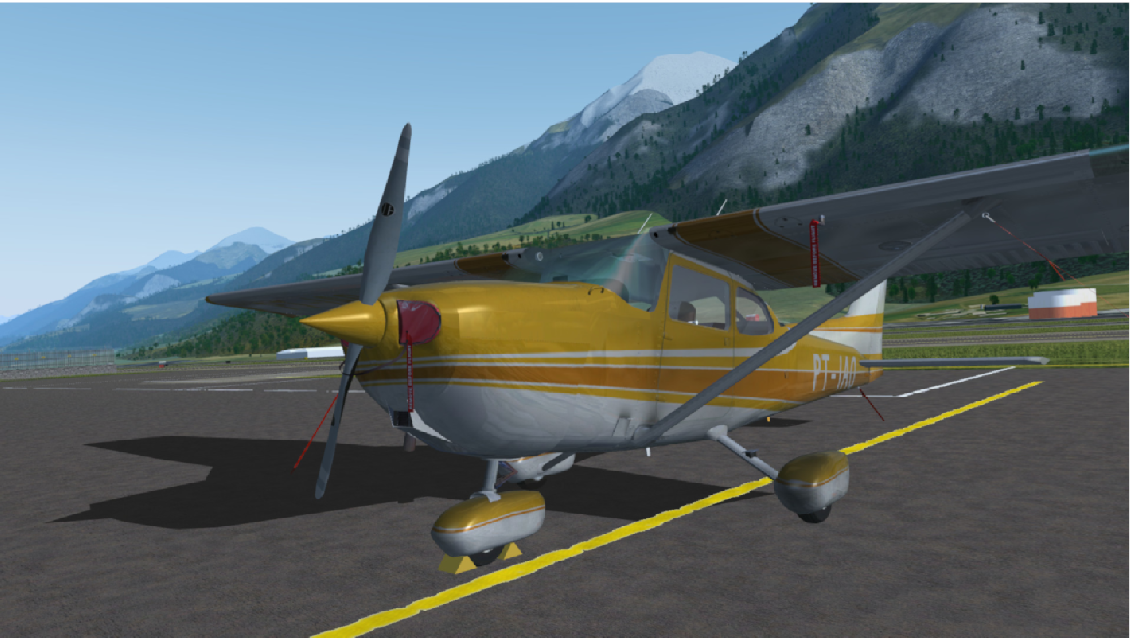
\includegraphics[clip,width=15.0cm]{img/cover}
 }}}}

\IfLanguageName{french}{
\date{Le manuel FlightGear\\
\today\\
Pour \FlightGear{} version \version{}}
}{}

\IfLanguageName{italian}{
\date{Manuale di FlightGear\\
\today\\
Per \FlightGear{} versione \version{}}
}{}

\IfLanguageName{english}{
\date{The FlightGear Manual\\
\today\\
For \FlightGear{} version \version{}}
}{}

\ifchinese
\date{FlightGear 手册\\
\today\\
适用于 \FlightGear{} \version{} 版\\
\small 佟辉(中文翻译)}
\fi

\maketitle
\noindent \small \textcolor{green}{关于封面图:}\\
\textbf{塞斯纳 172P 停在意大利奥斯塔山谷机场(LIMV)},由 Gilberto Agostinho 提供,GNU 通用公共许可证\\

\noindent 塞斯纳 172 天鹰(Skyhawk)是一种四座单引擎上单翼的固定翼飞机。于 1955 年首飞并一直生产畅销至今,塞斯纳 172 已是目前销量最大的飞机。\\

\noindent \textcolor{ForestGreen}{塞斯纳 172P 机模贡献者:}\\
David Megginson (原作者),\\
Gilberto Agostinho (gsagostinho), Wayne Bragg (wlbragg), Juan Vera del Campo (Juanvvc),\\
Daniel Dubreuil (Dany93), Jonathan Redpath (legoboyvdlp), Jonathan Schellhase (dg-505),\\
Tuomas Kuosmanen (tigert), Anders Gidenstam (AndersG), Waldo Kitty (wkitty42),\\
Jarl Arntzen (jarlarntzen), algefaen, Horacio, D-ECHO, onox, thevirtualfer
\vskip 5cm

\noindent \textcolor{blue}{此版本更新内容:}\\
第四章,启动器介绍,由 Stuart Buchanan 贡献\\
第八章,新的屏幕截图,由 Jonathan Redpath 贡献\\
第八章,转弯协调仪,由 Scott Giese 贡献\\


\tableofcontents

%% Revision 0.00  1998/09/08  michael
%% Initial revision for version 0.53.
%% revision 0.10  1998/10/01  michael
%% final proofreading for release
%% revision 0.11  1998/11/01  michael
%% added title pic
%% revision 0.3 2000/04/20 michael
%% Remark for tracing version
%% revision 0.5.2 2002/XX/XX michael
%% glad to add several new contributors
%% revision 0.6 2002/09/05 michael
%% changed title picture
%% revision 0.7 2005/10/29 Stuart Buchanan
%% add self to contributors and updated datestamp
